\section{LE5 -- Zentrale Aktoren \& Aktor-Gruppen finden}

\subsection{Ziel und Fragestellung}

Die Identifikation zentraler Aktoren in Netzwerken ist ein fundamentales Problem der Netzwerkanalyse. In unseren Fussballnetzwerken stellt sich die Frage: \textit{Welche Spieler oder Teams sind besonders wichtig für die Struktur und Funktion des Netzwerks?}

Die Antwort hängt stark von der Definition von \enquote{Zentralität} ab:
\begin{itemize}
  \item \textbf{Konnektivität}: Spieler mit vielen Verbindungen (Degree)
  \item \textbf{Brückenfunktion}: Spieler, die verschiedene Teamteile verbinden (Betweenness)
  \item \textbf{Erreichbarkeit}: Spieler mit kurzen Wegen zu allen anderen (Closeness)
  \item \textbf{Einfluss}: Spieler, die mit anderen wichtigen Spielern verbunden sind (Eigenvector, PageRank)
  \item \textbf{Gruppenzugehörigkeit}: Spieler in dicht verbundenen Kernen (k-Core)
\end{itemize}

In diesem Kapitel analysieren wir verschiedene Zentralitätsmasse auf unseren Pass- und Match-Netzwerken und identifizieren die wichtigsten Aktoren.

\subsection{Theoretische Grundlagen}

\subsubsection{Degree Centrality}

Die \textbf{Degree Centrality} $C_D(i)$ eines Knotens $i$ ist die einfachste Zentralitätsmass und zählt die Anzahl der direkten Verbindungen:

\begin{equation}
C_D(i) = \sum_{j} A_{ij}
\end{equation}

wobei $A$ die Adjazenzmatrix ist. Für ungerichtete Netzwerke ist dies einfach der Grad des Knotens.

\textbf{Normalisierte Degree Centrality}:
\begin{equation}
C_D^{norm}(i) = \frac{C_D(i)}{n-1}
\end{equation}

wobei $n$ die Anzahl der Knoten ist. Dies normalisiert die Zentralität auf den Bereich $[0,1]$.

Für \textbf{gerichtete Netzwerke} unterscheiden wir:
\begin{itemize}
  \item \textbf{In-Degree}: Anzahl eingehender Kanten (im Pass-Netzwerk: empfangene Pässe)
  \item \textbf{Out-Degree}: Anzahl ausgehender Kanten (im Pass-Netzwerk: gespielte Pässe)
\end{itemize}

Für \textbf{gewichtete Netzwerke} verwenden wir die \textbf{Strength} (gewichteter Degree):
\begin{equation}
s(i) = \sum_{j} w_{ij}
\end{equation}

wobei $w_{ij}$ das Gewicht der Kante zwischen $i$ und $j$ ist.

\subsubsection{Betweenness Centrality}

Die \textbf{Betweenness Centrality} misst, wie oft ein Knoten auf den kürzesten Pfaden zwischen anderen Knotenpaaren liegt:

\begin{equation}
C_B(i) = \sum_{s \neq i \neq t} \frac{\sigma_{st}(i)}{\sigma_{st}}
\end{equation}

wobei:
\begin{itemize}
  \item $\sigma_{st}$ = Anzahl kürzester Pfade von $s$ nach $t$
  \item $\sigma_{st}(i)$ = Anzahl dieser Pfade, die durch $i$ verlaufen
\end{itemize}

\textbf{Normalisierte Betweenness}:
\begin{equation}
C_B^{norm}(i) = \frac{2 \cdot C_B(i)}{(n-1)(n-2)}
\end{equation}

Knoten mit hoher Betweenness-Zentralität fungieren als \textbf{Brücken} oder \textbf{Broker} im Netzwerk. Ihre Entfernung kann das Netzwerk fragmentieren.

\subsubsection{Closeness Centrality}

Die \textbf{Closeness Centrality} misst, wie nah ein Knoten zu allen anderen Knoten ist:

\begin{equation}
C_C(i) = \frac{n-1}{\sum_{j \neq i} d(i,j)}
\end{equation}

wobei $d(i,j)$ die kürzeste Pfaddistanz von $i$ nach $j$ ist.

Knoten mit hoher Closeness-Zentralität können schnell alle anderen Knoten erreichen. Dies ist besonders in zusammenhängenden Komponenten relevant.

\textbf{Hinweis}: Für unzusammenhängende Netzwerke wird häufig die \textbf{Harmonic Centrality} verwendet, die mit reziproken Distanzen arbeitet.

\subsubsection{Eigenvector Centrality und PageRank}

Die \textbf{Eigenvector Centrality} bewertet Knoten nicht nur nach der Anzahl ihrer Verbindungen, sondern nach der Qualität dieser Verbindungen. Ein Knoten ist zentral, wenn er mit anderen zentralen Knoten verbunden ist.

Die Eigenvector-Zentralität $\mathbf{x}$ erfüllt:
\begin{equation}
\mathbf{x} = \lambda \mathbf{A} \mathbf{x}
\end{equation}

wobei $\lambda$ der grösste Eigenwert der Adjazenzmatrix $\mathbf{A}$ ist.

\textbf{PageRank} ist eine Variante für gerichtete Netzwerke mit einem Dämpfungsfaktor $\alpha$ (typischerweise 0.85):
\begin{equation}
PR(i) = \frac{1-\alpha}{n} + \alpha \sum_{j \to i} \frac{PR(j)}{deg^{out}(j)}
\end{equation}

PageRank modelliert einen Random Walk: Mit Wahrscheinlichkeit $\alpha$ folgt man einer ausgehenden Kante, mit Wahrscheinlichkeit $1-\alpha$ springt man zu einem zufälligen Knoten.

\subsubsection{k-Core und k-Shell}

Ein \textbf{k-Core} ist ein maximaler Subgraph, in dem jeder Knoten mindestens Grad $k$ innerhalb dieses Subgraphs hat.

Die \textbf{Core Number} (oder \textbf{Coreness}) eines Knotens ist das höchste $k$, für das der Knoten zum $k$-Core gehört.

Ein \textbf{k-Shell} enthält alle Knoten, die zum $k$-Core, aber nicht zum $(k+1)$-Core gehören.

k-Cores identifizieren hierarchisch strukturierte, dicht verbundene Gruppen im Netzwerk.

\subsection{Datengrundlage}

Wir analysieren folgende Netzwerke:
\begin{itemize}
  \item \textbf{Pass-Netzwerk (Deutschland)}: Knoten = Spieler, Kanten = Pässe (gerichtet, gewichtet)
  \item \textbf{Match-Netzwerk (World Cup)}: Knoten = Teams, Kanten = Spiele (gerichtet, gewichtet)
\end{itemize}

Für einige Zentralitätsmasse (Betweenness, Closeness, k-Core) verwenden wir die grösste zusammenhängende Komponente, um sinnvolle Ergebnisse zu erhalten.

\subsection{Ergebnisse: Pass-Netzwerk (Deutschland)}

\subsubsection{Degree Centrality und Strength}

Tabelle~\ref{tab:degree_stats} zeigt die Verteilungsstatistiken der Degree- und Strength-Werte im Pass-Netzwerk.

\begin{table}[htbp]
\centering
\caption{Degree und Strength Statistiken (Pass-Netzwerk Deutschland)}
\label{tab:degree_stats}
\begin{tabular}{lcc}
\toprule
\textbf{Metrik} & \textbf{Degree} & \textbf{Strength} \\
\midrule
Maximum & [aus Notebook] & [aus Notebook] \\
Mittelwert & [aus Notebook] & [aus Notebook] \\
Median & [aus Notebook] & [aus Notebook] \\
\bottomrule
\end{tabular}
\end{table}

Abbildung~\ref{fig:degree_dist} zeigt die Verteilung von Degree und Strength. Beide folgen einer typischen \textit{heavy-tailed} Verteilung: Die meisten Spieler haben wenige Verbindungen, während einige wenige sehr viele haben.

\begin{figure}[htbp]
  \centering
  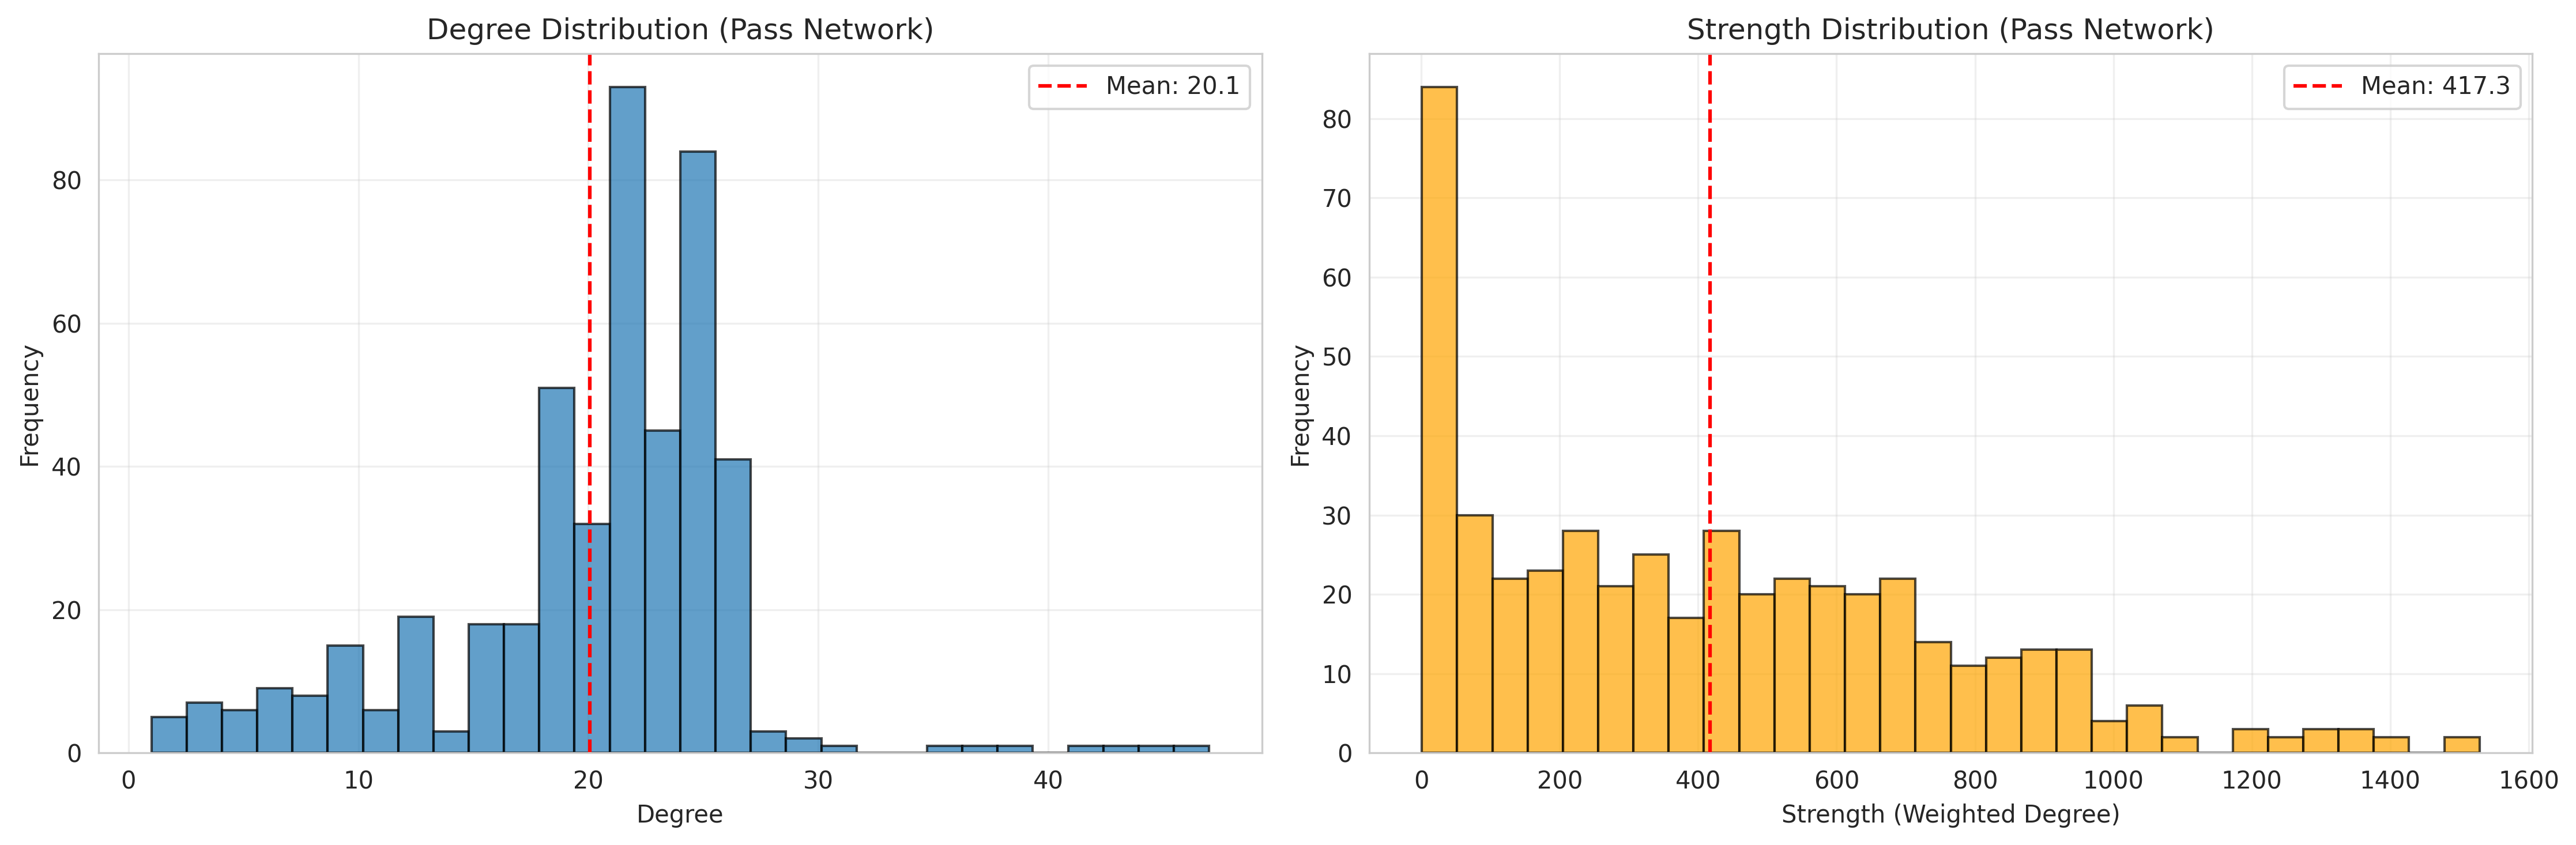
\includegraphics[width=0.95\textwidth]{figures/LE5/degree_distribution.png}
  \caption{Degree- und Strength-Verteilung im Pass-Netzwerk}
  \label{fig:degree_dist}
\end{figure}

Die Korrelation zwischen Degree und Strength ist sehr hoch ($r > 0.9$), was darauf hindeutet, dass Spieler mit vielen Verbindungen auch viele Pässe spielen.

\textbf{In-Degree vs. Out-Degree}: Im gerichteten Pass-Netzwerk zeigt sich:
\begin{itemize}
  \item Hoher \textbf{Out-Degree}: Spieler, die viele Pässe geben (Playmaker, Aufbauspieler)
  \item Hoher \textbf{In-Degree}: Spieler, die viele Pässe empfangen (Zielspieler, Stürmer)
\end{itemize}

\subsubsection{Betweenness Centrality}

Betweenness-Zentralität identifiziert Spieler, die als \textbf{Brücken} zwischen verschiedenen Teamteilen fungieren. Abbildung~\ref{fig:betweenness} zeigt die Verteilung und den Zusammenhang zwischen Degree und Betweenness.

\begin{figure}[htbp]
  \centering
  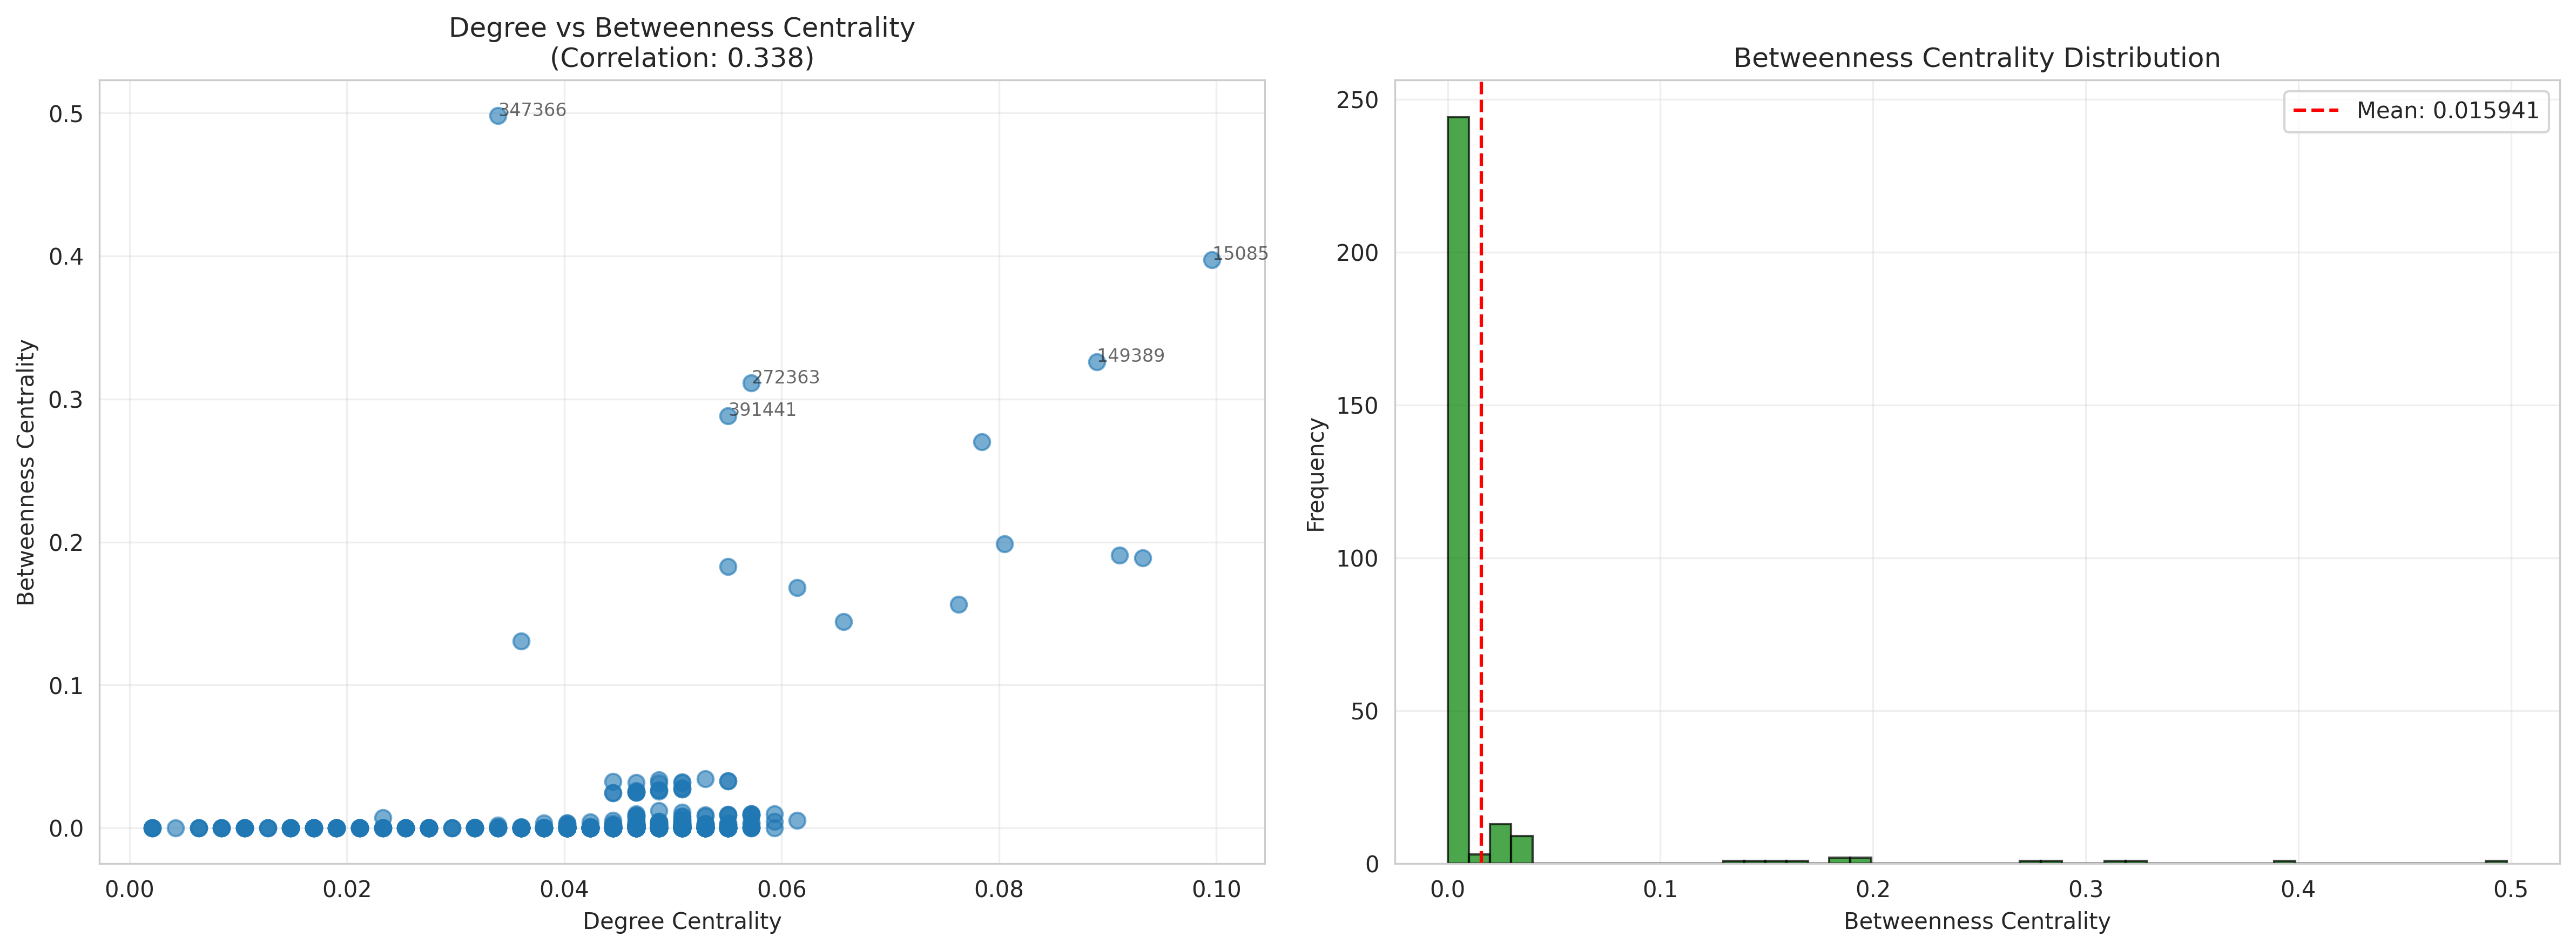
\includegraphics[width=0.95\textwidth]{figures/LE5/betweenness_analysis.png}
  \caption{Betweenness-Zentralität: Verteilung und Korrelation mit Degree}
  \label{fig:betweenness}
\end{figure}

Die Korrelation zwischen Degree und Betweenness ist moderat ($r \approx 0.5$--$0.7$), was bedeutet, dass nicht alle gut vernetzten Spieler auch Brückenfunktion haben.

\textbf{Bridging Nodes}: Spieler mit hoher Betweenness aber relativ niedrigem Degree sind besonders interessant – sie verbinden verschiedene Gruppen ohne selbst extrem viele Verbindungen zu haben. Diese Spieler sind strategisch wichtig für den Spielfluss.

\subsubsection{Vergleich aller Zentralitätsmasse}

Abbildung~\ref{fig:centrality_corr} zeigt die Korrelationsmatrix aller Zentralitätsmasse für das Pass-Netzwerk.

\begin{figure}[htbp]
  \centering
  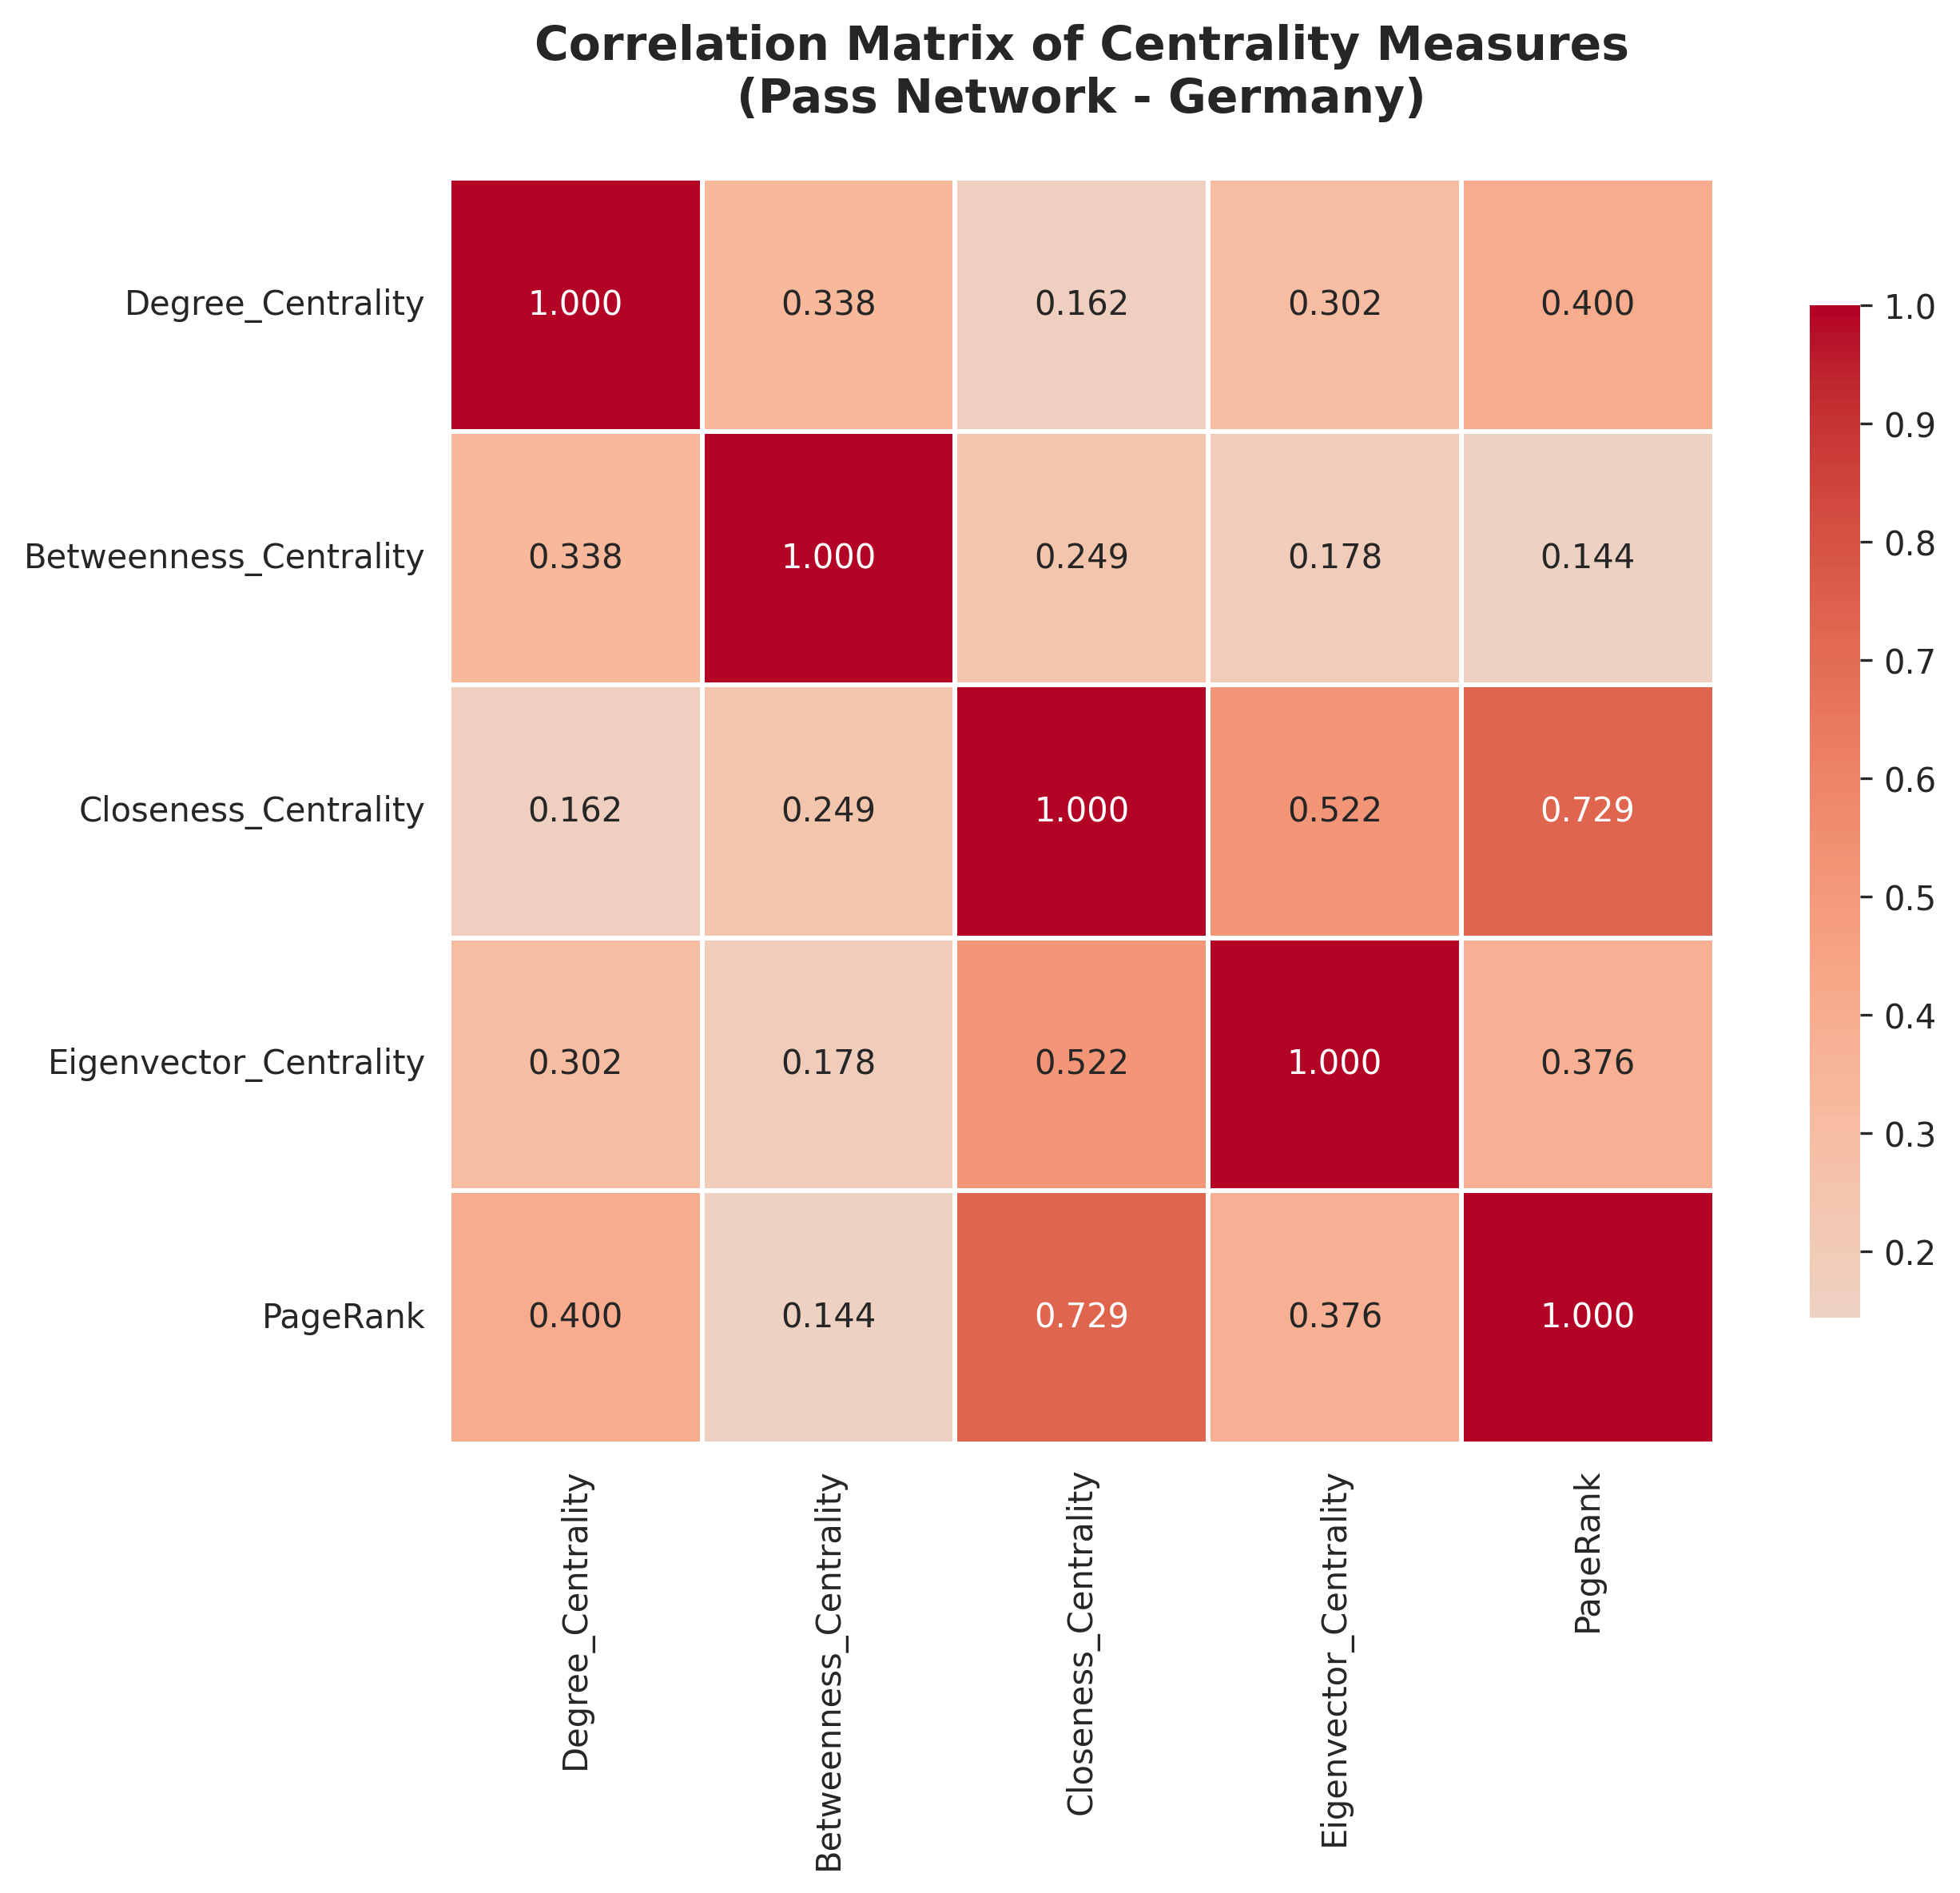
\includegraphics[width=0.8\textwidth]{figures/LE5/centrality_correlation.png}
  \caption{Korrelation verschiedener Zentralitätsmasse (Pass-Netzwerk)}
  \label{fig:centrality_corr}
\end{figure}

\textbf{Beobachtungen}:
\begin{itemize}
  \item \textbf{Degree, Eigenvector und PageRank} korrelieren stark miteinander ($r > 0.8$): Sie identifizieren ähnliche Spieler als zentral
  \item \textbf{Betweenness} korreliert schwächer mit den anderen Massen: Sie erfasst eine andere Dimension von Zentralität (Brückenfunktion)
  \item \textbf{Closeness} korreliert mässig mit allen anderen Massen
\end{itemize}

Dies zeigt, dass verschiedene Zentralitätsmasse verschiedene Aspekte der Wichtigkeit erfassen.

\subsubsection{Top Spieler nach Zentralität}

Tabelle~\ref{tab:top_players} zeigt die Top-10 Spieler nach durchschnittlichem Rang über alle Zentralitätsmasse.

\begin{table}[htbp]
\centering
\caption{Top-10 Spieler nach Gesamtzentralität (Pass-Netzwerk Deutschland)}
\label{tab:top_players}
\footnotesize
% Diese Tabelle wird aus dem Notebook generiert: top_players_table.tex
% Platzhalter für die tatsächlichen Daten
\begin{tabular}{lcccccc}
\toprule
\textbf{Spieler} & \textbf{Degree} & \textbf{Between.} & \textbf{Close.} & \textbf{PageRank} & \textbf{Core} & \textbf{Avg. Rank} \\
\midrule
284469 & 44 & 0.189000 & 0.241200 & 0.005000 & 18.000000 \\
15129 & 27 & 0.009800 & 0.231700 & 0.007300 & 18.000000 \\
14938 & 27 & 0.009300 & 0.231700 & 0.007400 & 18.000000 \\
14917 & 27 & 0.009300 & 0.231700 & 0.006500 & 18.000000 \\
14731 & 38 & 0.198800 & 0.257500 & 0.004500 & 18.000000 \\
15775 & 26 & 0.009700 & 0.231500 & 0.008900 & 18.000000 \\
16094 & 43 & 0.190900 & 0.232700 & 0.004600 & 20.000000 \\
15191 & 27 & 0.009300 & 0.231700 & 0.006000 & 18.000000 \\
25861 & 26 & 0.009000 & 0.231500 & 0.007800 & 18.000000 \\
14778 & 26 & 0.183100 & 0.256800 & 0.007000 & 19.000000 \\\bottomrule
\end{tabular}
\end{table}

\subsection{k-Core Analyse}

Die k-Core-Zerlegung identifiziert hierarchische Struktur im Netzwerk. Abbildung~\ref{fig:kcore} zeigt die Verteilung der Core-Nummern und deren Zusammenhang mit Degree.

\begin{figure}[htbp]
  \centering
  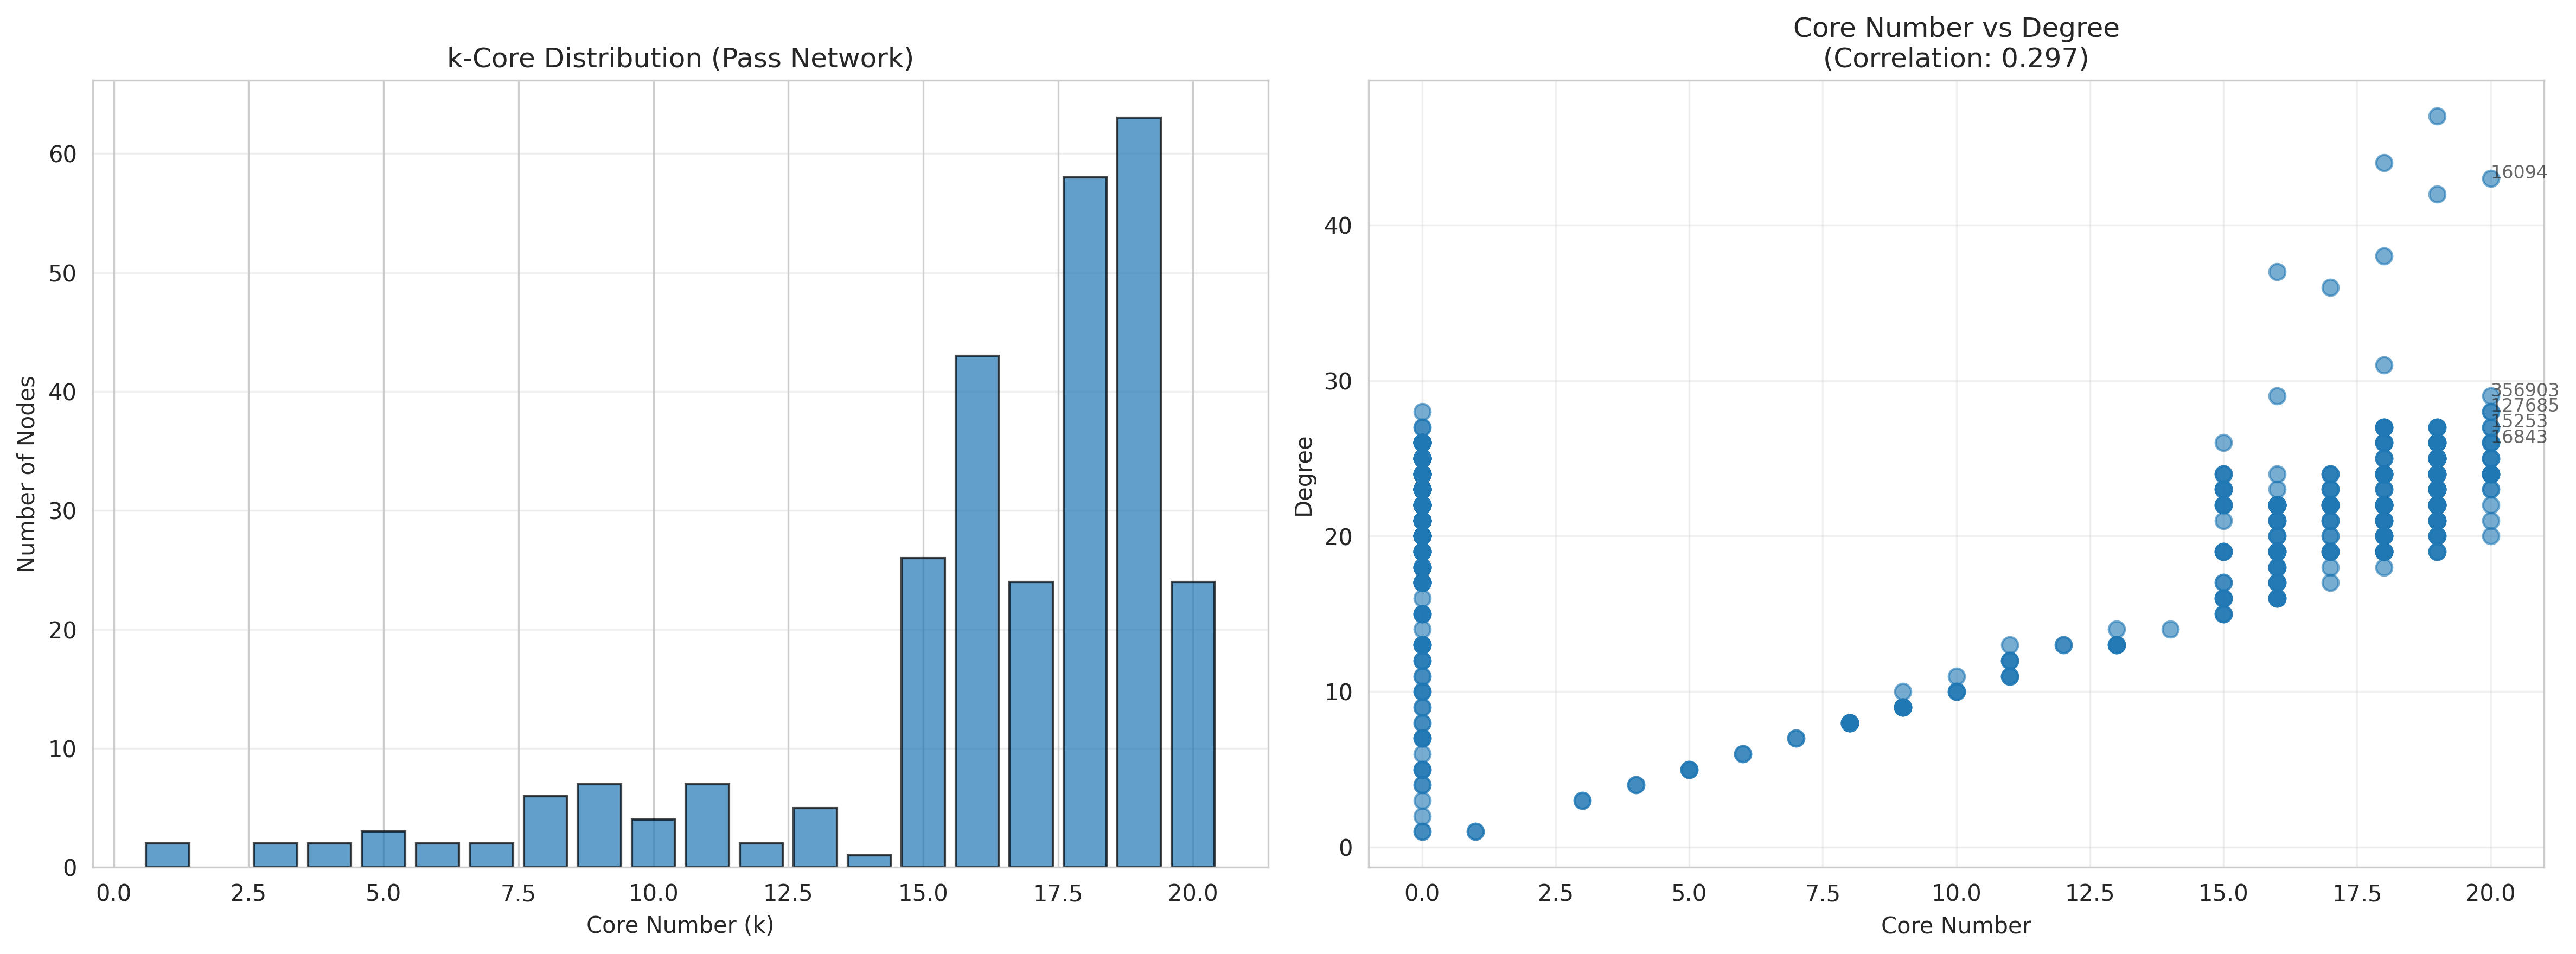
\includegraphics[width=0.95\textwidth]{figures/LE5/kcore_analysis.png}
  \caption{k-Core Analyse: Verteilung und Zusammenhang mit Degree}
  \label{fig:kcore}
\end{figure}

\textbf{Interpretation}:
\begin{itemize}
  \item Der \textbf{maximale Core} (höchster $k$-Wert) enthält die am dichtesten verbundene Gruppe von Spielern
  \item Die starke Korrelation zwischen Core Number und Degree ($r > 0.9$) zeigt, dass Spieler mit vielen Verbindungen typischerweise in höheren Cores sind
  \item Spieler im höchsten Core bilden das \enquote{Backbone} des Pass-Netzwerks
\end{itemize}

Die k-Core-Analyse ergänzt die punktbasierten Zentralitätsmasse, indem sie \textbf{Gruppen} von dicht verbundenen Spielern identifiziert.

\subsection{Ergebnisse: Match-Netzwerk (World Cup)}

\subsubsection{Team-Zentralität}

Im Match-Netzwerk repräsentieren Knoten Teams und Kanten Spiele. Die Analyse der Zentralität identifiziert die wichtigsten Teams im Wettbewerb.

Abbildung~\ref{fig:centrality_corr_match} zeigt die Korrelationsmatrix für das Match-Netzwerk.

\begin{figure}[htbp]
  \centering
  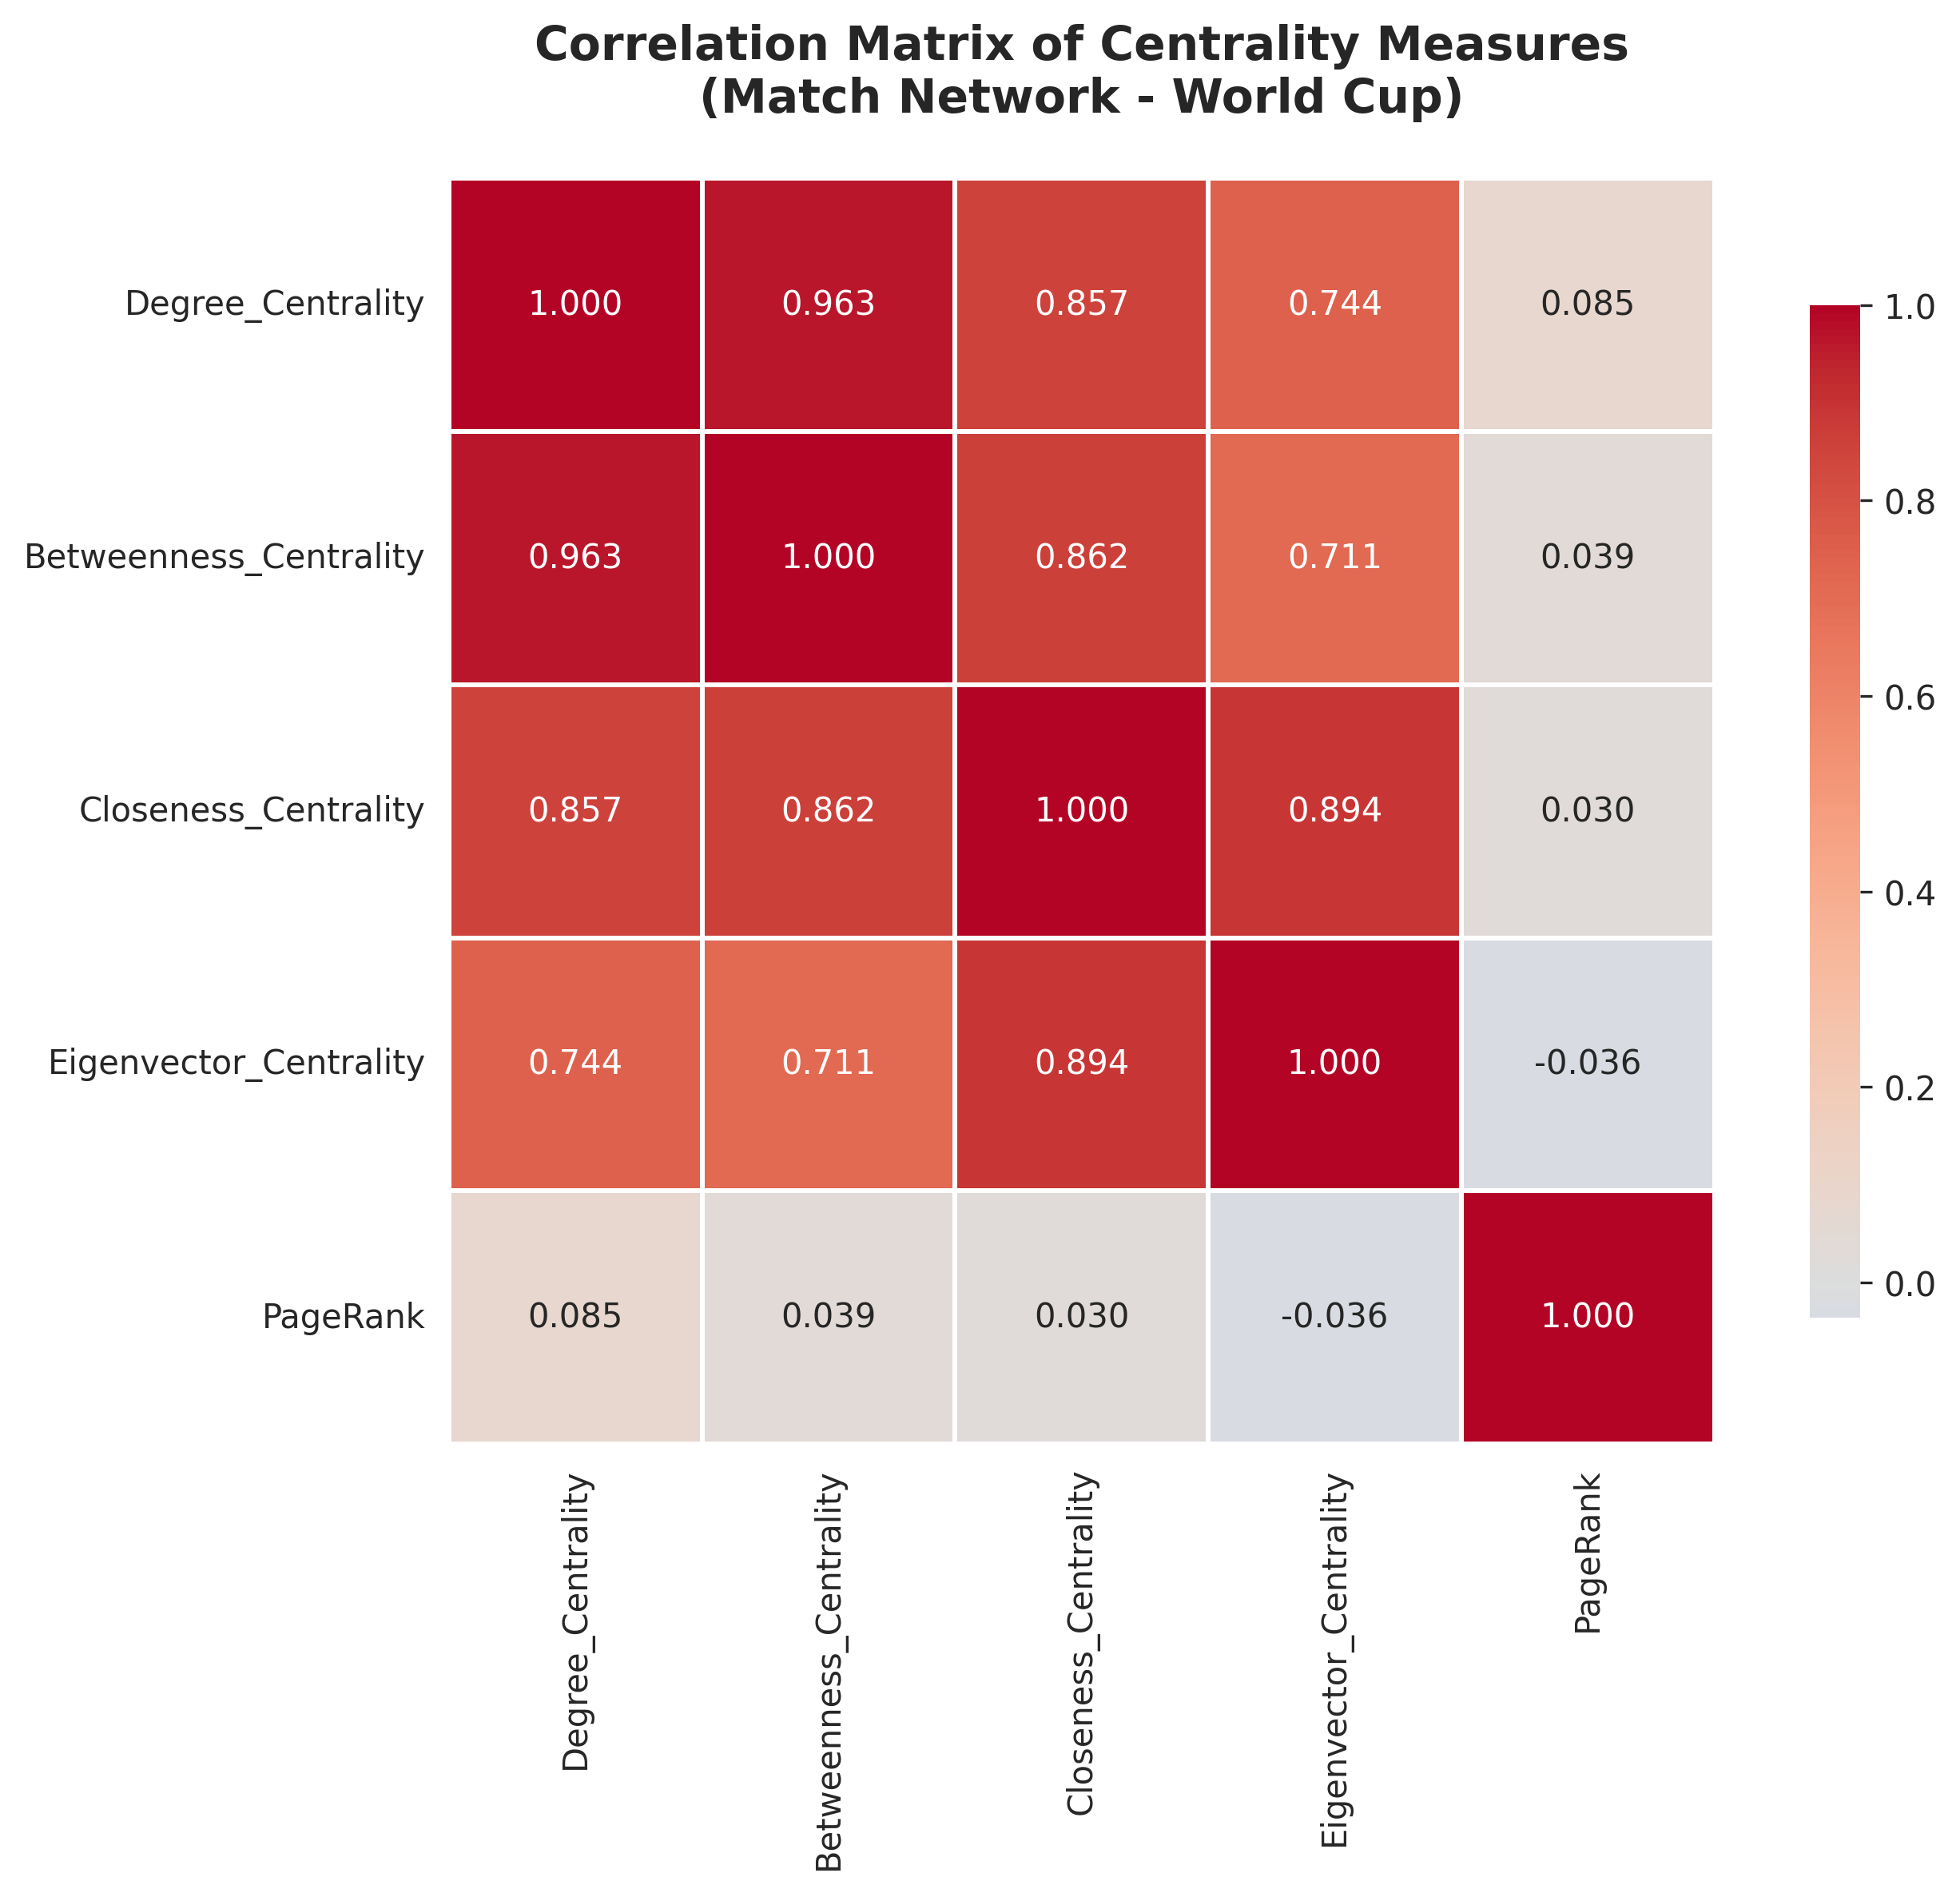
\includegraphics[width=0.8\textwidth]{figures/LE5/centrality_correlation_match.png}
  \caption{Korrelation verschiedener Zentralitätsmasse (Match-Netzwerk World Cup)}
  \label{fig:centrality_corr_match}
\end{figure}

\textbf{Beobachtungen}:
\begin{itemize}
  \item Im Match-Netzwerk sind die Korrelationen zwischen verschiedenen Zentralitätsmassen tendenziell höher als im Pass-Netzwerk
  \item Dies deutet auf eine homogenere Struktur hin: Teams, die viele Spiele haben, sind auch zentral nach anderen Massen
  \item Die höchsten Zentralitätswerte haben typischerweise Teams, die weit im Turnier gekommen sind (mehr Spiele = höhere Zentralität)
\end{itemize}

\subsection{Vergleich: Pass-Netzwerk vs. Match-Netzwerk}

Die beiden Netzwerktypen zeigen unterschiedliche Strukturen:

\begin{itemize}
  \item \textbf{Pass-Netzwerk}: Komplexere Struktur mit verschiedenen Spielerrollen (Verteidiger, Mittelfeld, Angriff), stärkere Heterogenität in Zentralitätsmassen
  \item \textbf{Match-Netzwerk}: Struktur stark vom Turnierformat geprägt (K.O.-System, Gruppenphase), höhere Korrelation zwischen Zentralitätsmassen
\end{itemize}

\subsection{Interpretation und Diskussion}

\subsubsection{Verschiedene Zentralitäten erfassen verschiedene Rollen}

Unsere Analyse zeigt, dass verschiedene Zentralitätsmasse verschiedene Aspekte von Wichtigkeit erfassen:

\begin{itemize}
  \item \textbf{Degree/Strength}: Aktivität und Beteiligung (viele Pässe spielen/empfangen)
  \item \textbf{Betweenness}: Strategische Position (Brückenfunktion zwischen Teamteilen)
  \item \textbf{Closeness}: Integration (kurze Wege zu allen Mitspielern)
  \item \textbf{Eigenvector/PageRank}: Einfluss (Verbindung zu wichtigen Spielern)
  \item \textbf{k-Core}: Zugehörigkeit zu dicht verbundenen Gruppen
\end{itemize}

Je nach analytischem Ziel sollte das passende Zentralitätsmass gewählt werden.

\subsubsection{Spielerrollen im Fussball}

Die Zentralitätsmasse können helfen, verschiedene Spielerrollen zu identifizieren:
\begin{itemize}
  \item \textbf{Playmaker}: Hoher Degree, hoher PageRank (viele Pässe, verbunden mit wichtigen Spielern)
  \item \textbf{Brückenspieler}: Hohe Betweenness, moderater Degree (verbinden verschiedene Mannschaftsteile)
  \item \textbf{Core-Spieler}: Hohe Core Number (Teil des zentralen Spielsystems)
\end{itemize}

\subsubsection{Normalisierung und Vergleichbarkeit}

Die Normalisierung von Zentralitätsmassen ist wichtig für den Vergleich über verschiedene Netzwerke hinweg:
\begin{itemize}
  \item \textbf{Normalisierte Degree Centrality}: Berücksichtigt Netzwerkgrösse
  \item \textbf{Normalisierte Betweenness}: Macht Werte über verschiedene Netzwerke vergleichbar
  \item Ohne Normalisierung würden grössere Netzwerke systematisch höhere Zentralitätswerte produzieren
\end{itemize}

\subsubsection{Limitationen}

Einige Einschränkungen unserer Analyse:
\begin{itemize}
  \item \textbf{Closeness} ist nur in zusammenhängenden Komponenten sinnvoll
  \item \textbf{Betweenness} ist rechenintensiv für grosse Netzwerke
  \item Zentralitätsmasse berücksichtigen nicht die \textbf{Qualität} der Aktionen (z.B. erfolgreiche vs. erfolglose Pässe)
  \item Zeitliche Dynamik wird nicht erfasst (statische Netzwerkansicht)
\end{itemize}

\subsection{Fazit}

Die Analyse der Aktorzentralität offenbart wichtige strukturelle Eigenschaften der Fussballnetzwerke:

\begin{enumerate}
  \item \textbf{Heterogenität}: Einige wenige Spieler/Teams sind deutlich zentraler als andere
  \item \textbf{Multidimensionalität}: Verschiedene Zentralitätsmasse identifizieren teilweise verschiedene Aktoren als wichtig
  \item \textbf{Rollen-Identifikation}: Kombinationen von Zentralitätsmassen können helfen, funktionale Rollen zu identifizieren
  \item \textbf{Strategische Wichtigkeit}: Knoten mit hoher Betweenness sind strategisch wichtig für den Informations-/Passfluss
  \item \textbf{Kohäsive Gruppen}: k-Core-Analyse ergänzt punktbasierte Masse durch Gruppenperspektive
\end{enumerate}

Diese Erkenntnisse sind sowohl für die deskriptive Netzwerkanalyse als auch für strategische Überlegungen (z.B. welche Spieler sind am wichtigsten für das Team?) relevant.

\textbf{Ausblick}: In weiteren Analysen könnten dynamische Zentralitätsmasse (wie sich Zentralität über Zeit ändert) oder positions-spezifische Zentralität (getrennt nach Spielpositionen) untersucht werden.
